% ============================================================================
% FILE: sections/05_test_results.tex
% PURPOSE: ผลการทดสอบ Unit Test และ System Test แยกตาม Progress
% ============================================================================

\section{ผลการทดสอบ (Test Results)}

% ============================================================
\subsection{ผลการทดสอบ Progress Update 1}
% ============================================================

\subsubsection{ผล FEA และการคำนวณ Deflection}
% อ้างอิง M3: $\delta_{\text{total}} = 0.237$ mm $< 1$ mm --- ผ่าน

\begin{table}[H]
  \centering
  \caption{ผล FEA เทียบกับเกณฑ์ M3}
  \label{tab:fea_p1}
  % [ตาราง: วิธี | delta (mm) | เกณฑ์ | ผล]
\end{table}

\subsubsection{ผลการคำนวณ Motion Profile (ทฤษฎี)}
% อ้างอิง P1: เวลารวม = 34.39 s < 35 s --- ผ่านในทฤษฎี

% ============================================================
\subsection{ผลการตรวจสอบความถูกต้องของแบบจำลอง (Model Validation)}
\label{subsec:model_validation_results}
% ============================================================

ในหัวข้อนี้แสดงผลการตรวจสอบความถูกต้องของแบบจำลอง (Transfer Function) ที่ได้จากการทำ System Identification โดยเปรียบเทียบระหว่างสัญญาณความเร็วเชิงมุมที่วัดได้จริงจาก Hardware ($y_{measured}$) กับสัญญาณที่ได้จากการ Simulate แบบจำลอง ($y_{simulated}$) ภายใต้สัญญาณ Excitation รูปแบบต่าง ๆ

\begin{figure}[H]
  \centering
  
\includegraphics[width=0.88\textwidth]{images/chirp_raw_filtered.png}
  \caption{สัญญาณ Chirp ก่อนและหลัง Filter (chirp1\_run1) แสดง $V_{in}$ และ $\omega_{arm}$}
  \label{fig:chirp_filtered}
\end{figure}

\begin{figure}[H]
  \centering
  
\includegraphics[width=1\textwidth]{images/cross_validation.png}
  \caption{เปรียบเทียบ Measured กับ Simulated สำหรับ Stair-Step data (3 runs)}
  \label{fig:cross_val}
\end{figure}

\begin{figure}[H]
  \centering
  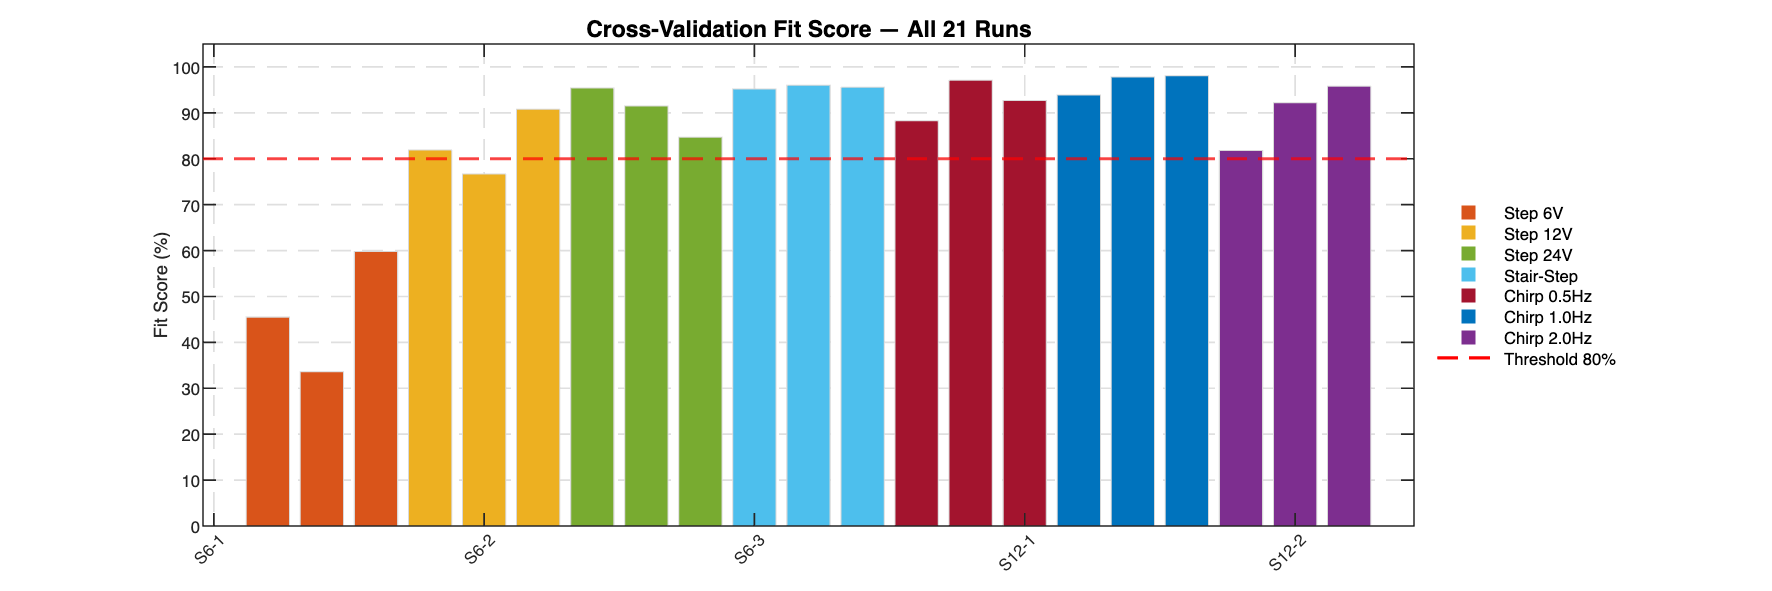
\includegraphics[width=0.88\textwidth]{images/cross_val_bar.png}
  \caption{Fit Score จาก Cross-Validation กับข้อมูลประเภทต่าง ๆ ทั้ง 21 runs
           (เส้นประแดงคือเกณฑ์ 80\%)}
  \label{fig:cross_val_bar}
\end{figure}

\begin{table}[H]
  \centering
  \caption{ผลการ Cross-Validation ของ Model กับข้อมูลประเภทต่าง ๆ}
  \label{tab:cross_val_result}
  \begin{tabular}{lcccc}
    \toprule
    ชุดข้อมูล & Fit Score (\%) & Std (\%) & NRMSE (\%) & ผลการประเมิน \\
    \midrule
    Chirp 0.1--0.5\,Hz (3 runs) & 92.7 & 4.4  & 7.3  & ผ่าน \\
    Chirp 0.1--1.0\,Hz (3 runs) & 96.6 & 2.3  & 3.4  & ผ่าน \\
    Chirp 0.1--2.0\,Hz (3 runs) & 89.9 & 7.3  & 10.1 & ผ่าน \\
    Step 6\,V (3 runs)          & 46.3 & 13.1 & 53.7 & \textbf{ไม่ผ่าน} \\
    Step 12\,V (3 runs)         & 83.1 & 7.1  & 16.9 & ผ่าน \\
    Step 24\,V (3 runs)         & 90.5 & 5.4  & 9.5  & ผ่าน \\
    Stair-Step (3 runs)         & 95.6 & 0.4  & 4.4  & ผ่านดีมาก \\
    \bottomrule
  \end{tabular}
\end{table}

% ============================================================
\subsection{ผลการจำลองสมรรถนะการควบคุม (Control Performance Simulation)}
\label{subsec:sim_results_arm}
% ============================================================

หัวข้อนี้แสดงผลการประเมินสมรรถนะของ Cascade PID Controller ร่วมกับ S-Curve Motion Profile ผ่านการ Simulation โดยใช้พารามิเตอร์ที่ออกแบบไว้ในบทที่ 2

\begin{figure}[H]
  \centering
  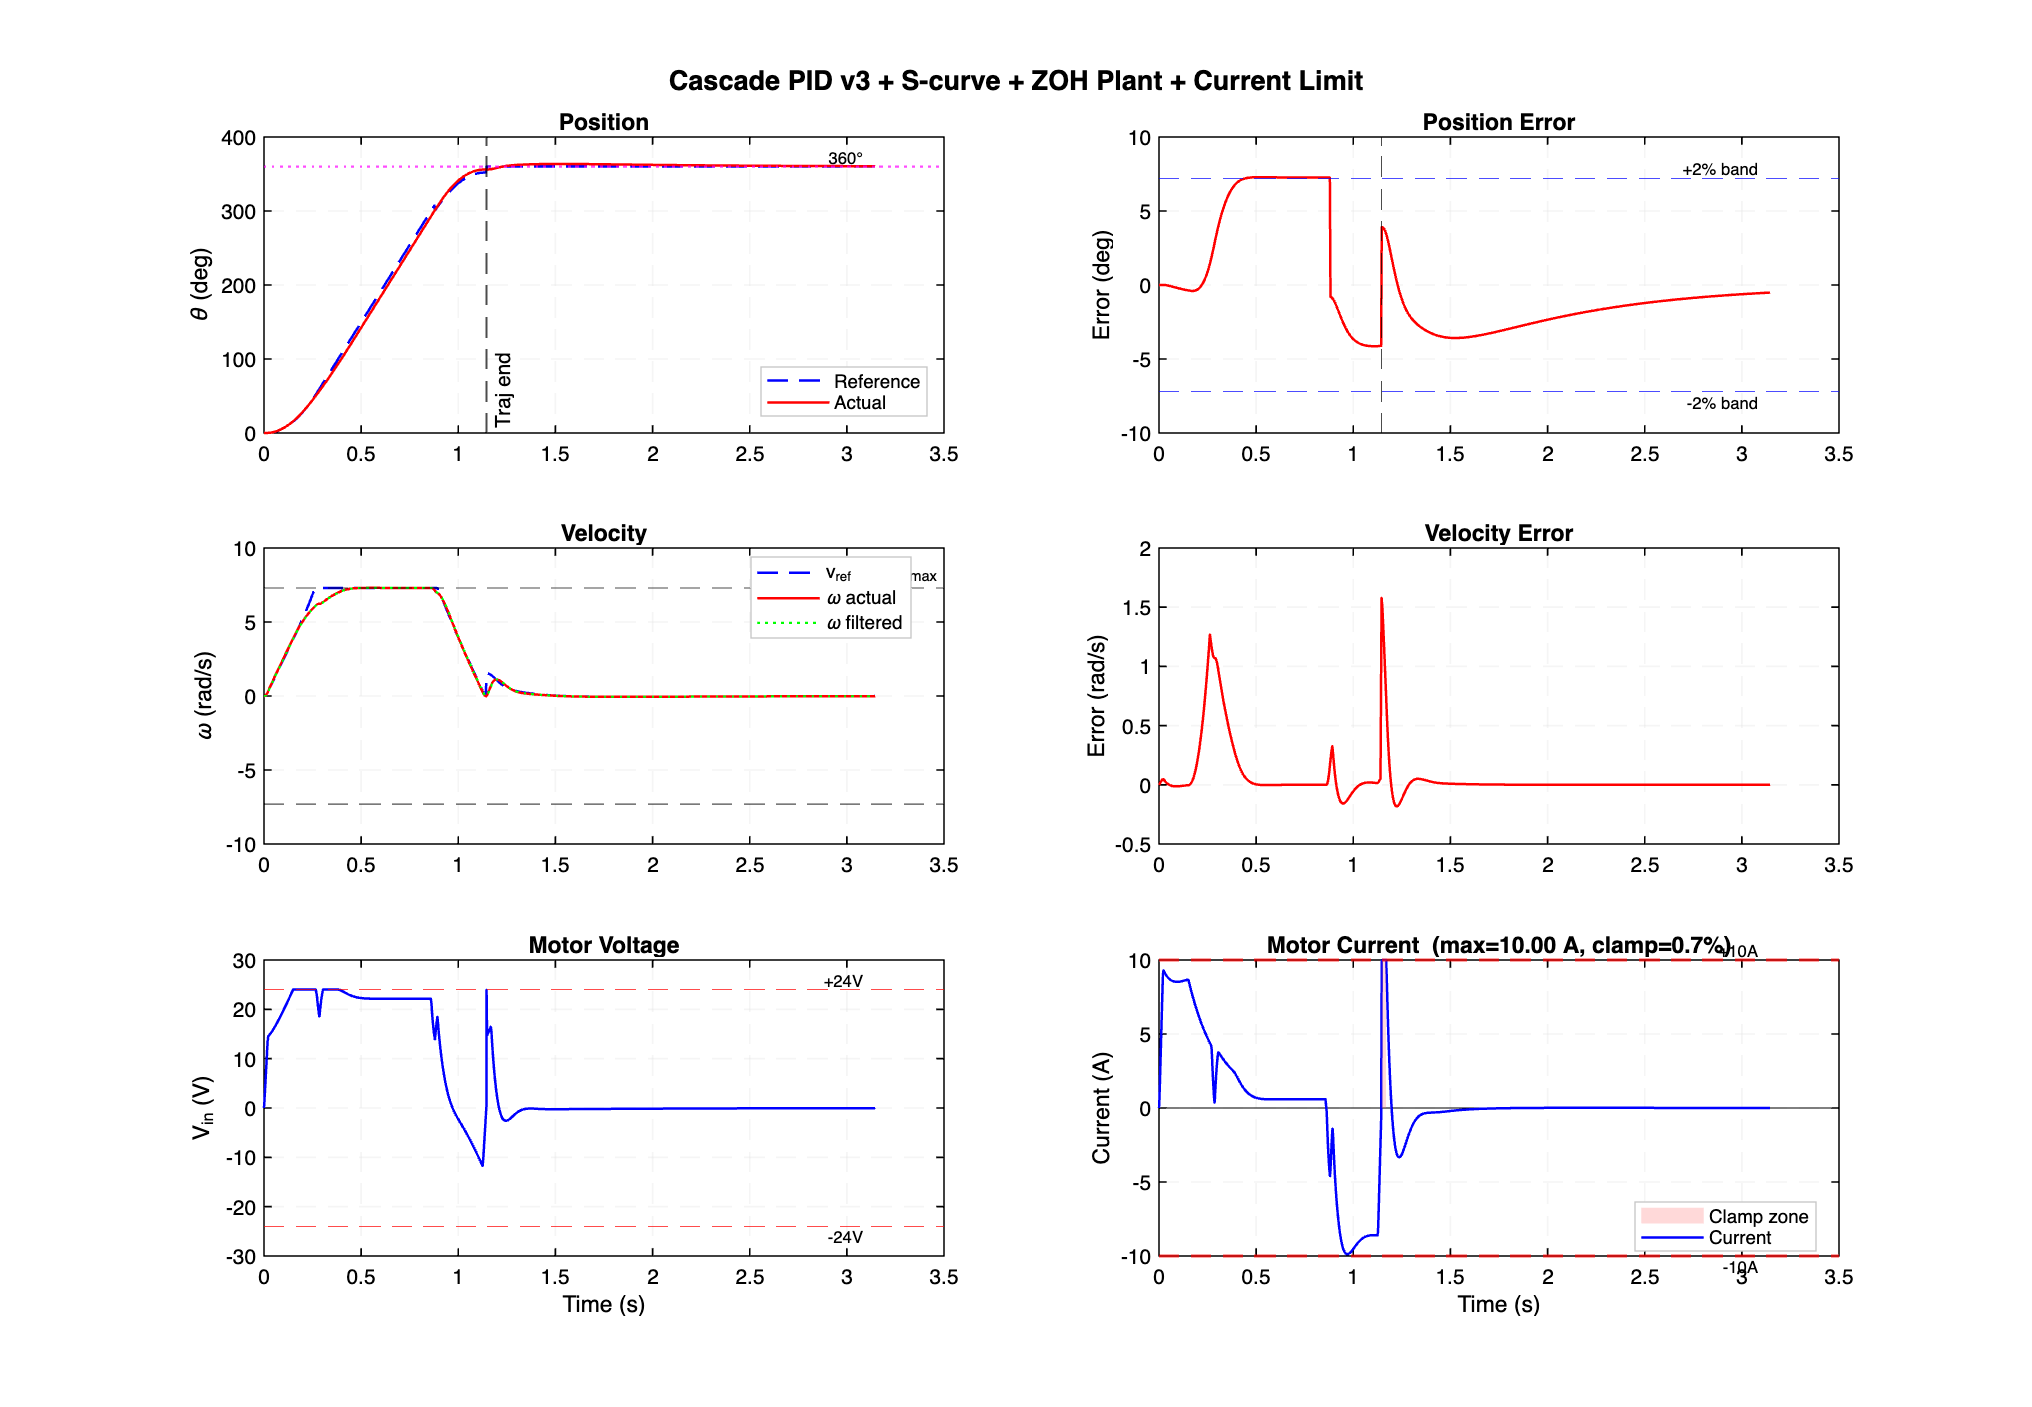
\includegraphics[width=0.95\textwidth]{images/sim_result.png}
  \caption{ผล Simulation: Position, Position Error, Velocity, Velocity Error,
           Motor Voltage และ Motor Current (S-Curve 360°, Cascade PID)}
  \label{fig:sim_result}
\end{figure}

\begin{figure}[H]
  \centering
  
\includegraphics[width=0.78\textwidth]{images/sim_current.png}
  \caption{Motor Current และ Current Clamp Zone ระหว่างการเคลื่อนที่ 360°}
  \label{fig:sim_current}
\end{figure}

\begin{table}[H]
  \centering
  \caption{ผล Simulation เทียบกับ Requirement (S-Curve 360°)}
  \label{tab:sim_vs_req}
  \begin{tabular}{lcccc}
    \toprule
    พารามิเตอร์ & ผล Simulation & Requirement & หน่วย & ผลการตรวจสอบ \\
    \midrule
    Settling Time       & 0.0198  & $\leq 0.5$ & s   & ผ่าน \\
    Overshoot           & 0.9948  & $\leq 1$   & \%  & ผ่าน \\
    Steady-state Error  & 0.512   & --         & deg & -- \\
    Max Current         & 10.00   & $\leq 10$  & A   & ผ่าน \\
    Current Clamp       & 0.71    & --         & \%  & -- \\
    Move Time (360°)    & 1.146   & --         & s   & -- \\
    Cycle Time (4 pcs)  & 22.58   & $\leq 35$  & s   & ผ่าน \\
    \bottomrule
  \end{tabular}
\end{table}

% ============================================================
\subsection{ผลการวิเคราะห์และหาค่าพารามิเตอร์ที่เหมาะสม (Optimization Results)}
\label{subsec:rod_opt_results}
% ============================================================

ผลการวิเคราะห์ Multi-objective Optimization ด้วย NSGA-II เพื่อหาจุดที่เหมาะสมที่สุด (Optimal Solution) ระหว่างเวลาในการทำงาน (Cycle Time) และการแกว่งของชิ้นงาน (Rod Swing)

\begin{figure}[H]
  \centering
  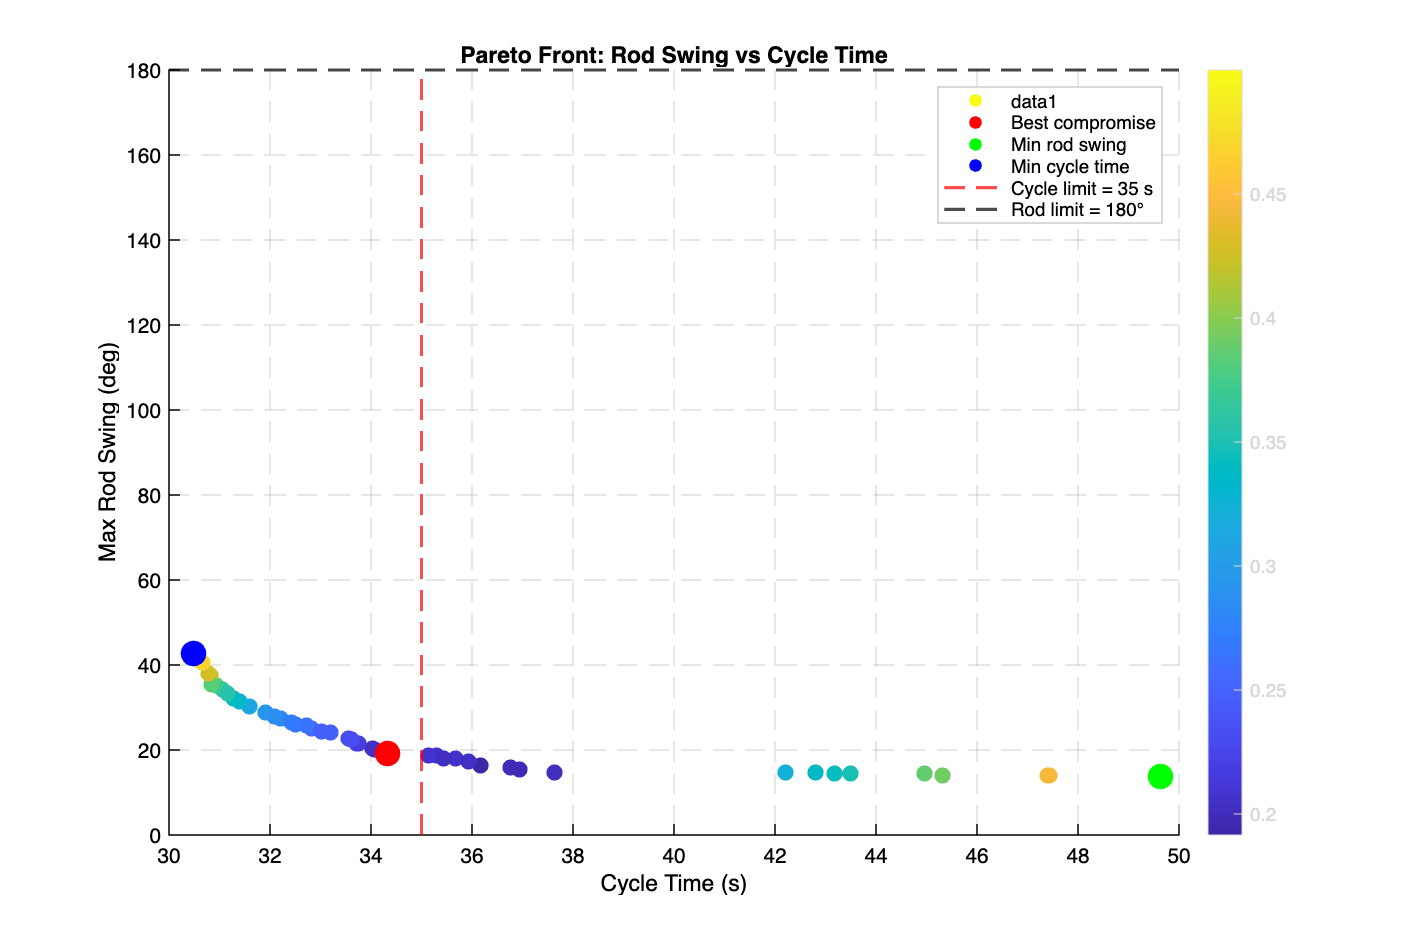
\includegraphics[width=0.88\textwidth]{images/pareto_front.png}
  \caption{Pareto Front จาก NSGA-II แสดง Trade-off ระหว่าง
           Max Rod Swing และ Cycle Time}
  \label{fig:pareto_front}
\end{figure}

\begin{table}[H]
  \centering
  \caption{สรุป Solution บน Pareto Front ที่น่าสนใจ}
  \label{tab:pareto_summary}
  \begin{tabular}{lcccl}
    \toprule
    Solution & Rod Swing (deg) & Cycle Time (s) & ผ่าน 35\,s & หมายเหตุ \\
    \midrule
    ไม่มี Shaping (เดิม)            & 198.0 & $\infty$ & ไม่ผ่าน & Rod ไม่นิ่ง \\
    ZV Shaping (พารามิเตอร์เดิม)   & 84.4  & $\infty$ & ไม่ผ่าน & Rod ไม่นิ่ง \\
    Min Cycle Time                  & 42.7  & 30.5     & ผ่าน    & Rod swing สูง \\
    Best Compromise                 & 19.1  & 34.3     & ผ่าน    & สมดุลดีที่สุด \\
    Min Rod Swing                   & 13.8  & 49.6     & \textbf{ไม่ผ่าน} & เกิน 35\,s มาก \\
    \bottomrule
  \end{tabular}
\end{table}

Solution ที่เลือกใช้คือ ``Best Compromise'' ซึ่งให้ค่าพารามิเตอร์สำหรับการเคลื่อนที่ดังตารางที่~\ref{tab:opt_params} และผลตอบสนองเชิงเวลาดังรูปที่~\ref{fig:rod_best_compromise}

\begin{table}[H]
  \centering
  \caption{ค่าพารามิเตอร์ที่ Optimal จาก NSGA-II (Best Compromise)}
  \label{tab:opt_params}
  \begin{tabular}{lcc}
    \toprule
    พารามิเตอร์ & ค่า & หน่วย \\
    \midrule
    $v_{max}$           & 4.856  & rad/s \\
    $a_{max}$           & 5.960  & rad/s$^2$ \\
    $j_{max}$           & 1085.9 & rad/s$^3$ \\
    $\omega_{n,shaper}$ & 12.386 & rad/s \\
    $\zeta_{shaper}$    & 0.0984 & -- \\
    \midrule
    Rod Swing           & 19.1   & deg \\
    Cycle Time          & 34.3   & s \\
    Arm Settling Time   & 0.067  & s \\
    Overshoot           & 0.018  & \% \\
    Max Current         & 3.62   & A \\
    \bottomrule
  \end{tabular}
\end{table}

\begin{figure}[H]
  \centering
  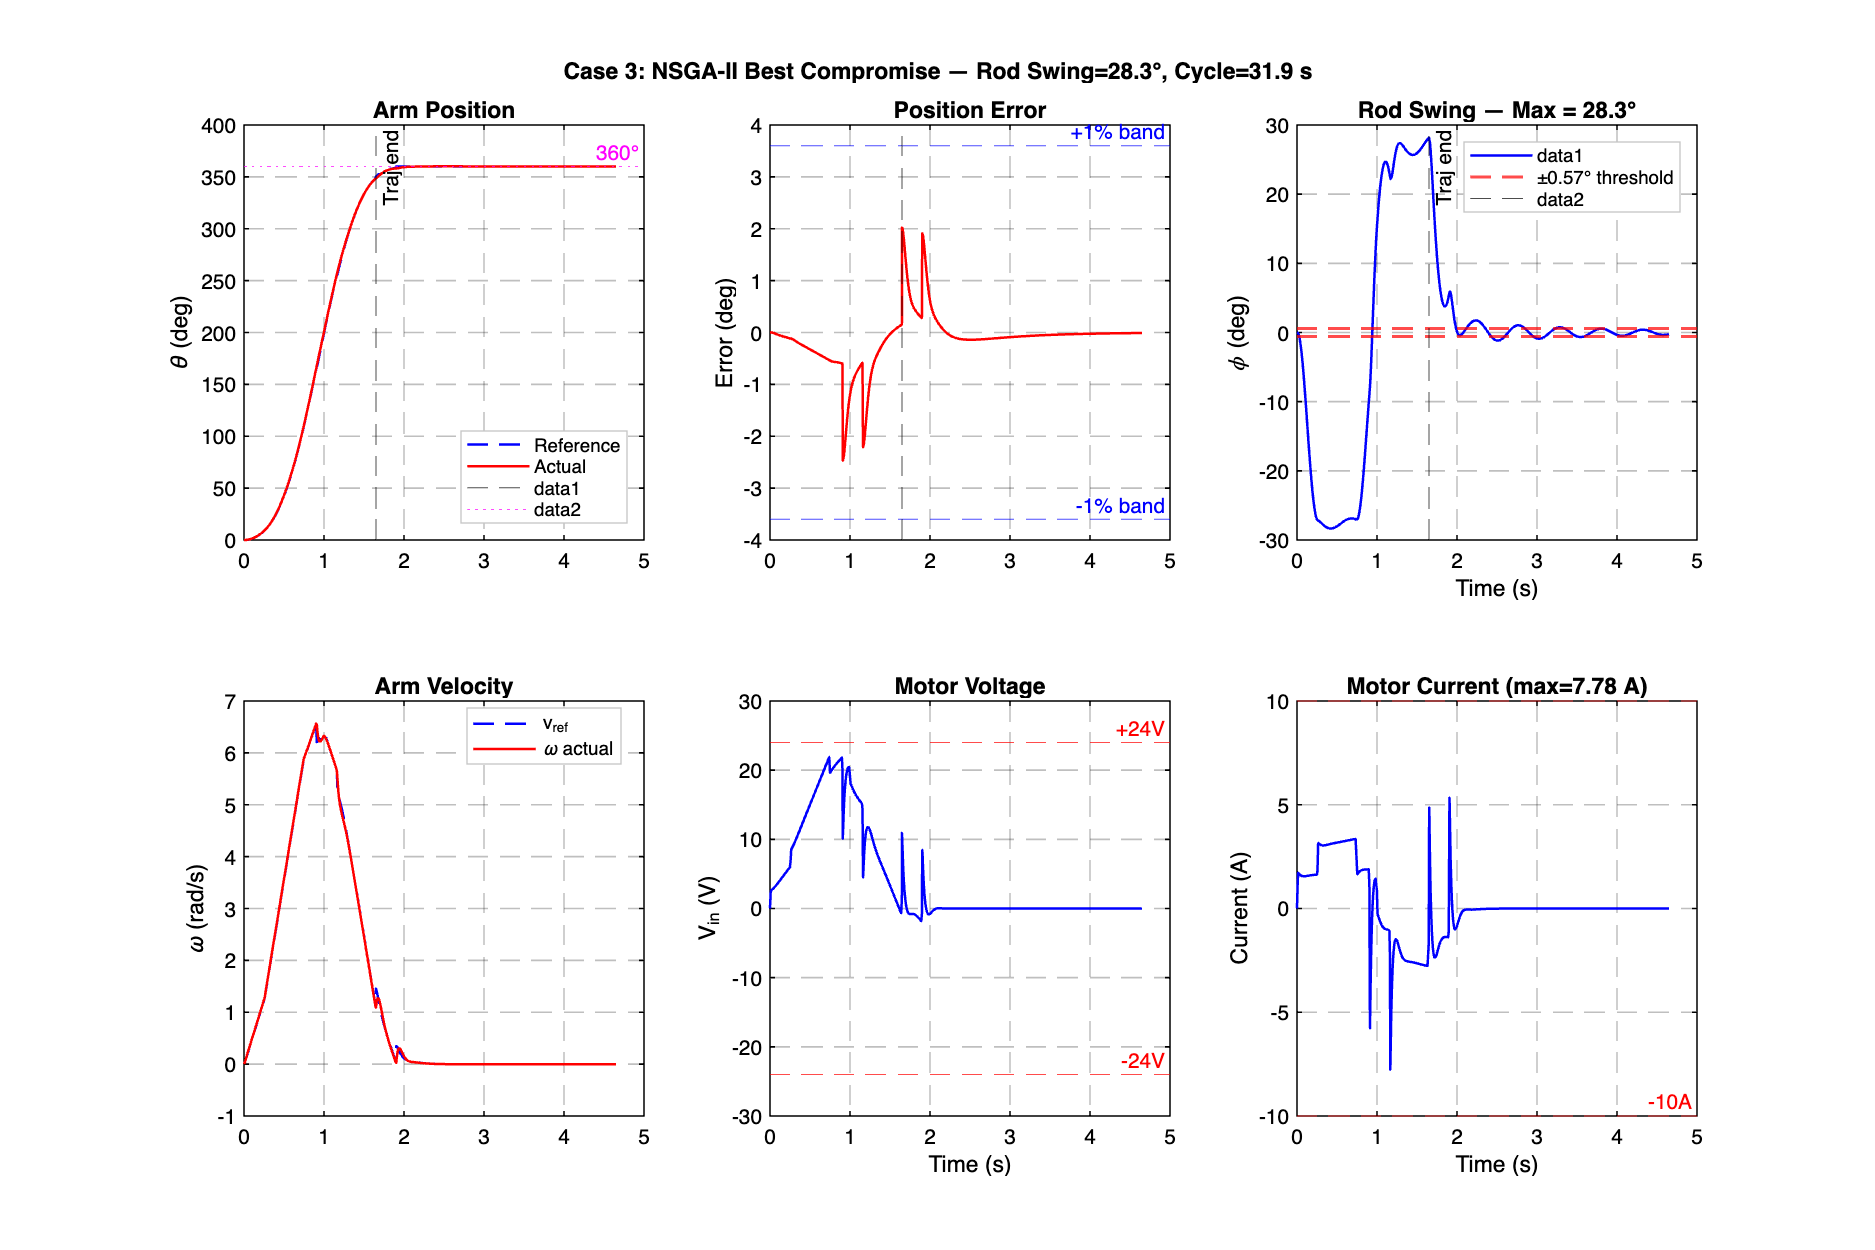
\includegraphics[width=0.88\textwidth]{images/rod_best_compromise.png}
  \caption{ผล Simulation ของ Best Compromise Solution จาก NSGA-II
           (Rod Swing = 19.1°, Cycle Time = 34.3\,s)}
  \label{fig:rod_best_compromise}
\end{figure}

% ============================================================
\subsection{ผลการทดสอบ Progress Update 2 (Unit Tests)}
% ============================================================

\subsubsection{Unit Test: การอ่าน Encoder และ PWM (Deliverable 2)}
...

\begin{table}[H]
  \centering
  \caption{ผล Unit Test Joystick แต่ละโหมด}
  \label{tab:joystick_unit_test}
  % [ตาราง: โหมด | ปุ่มที่กด | การตอบสนอง | Pass/Fail]
\end{table}

\subsubsection{Unit Test: ตู้ควบคุมไฟฟ้า (Deliverable 1)}
% สถานะ: กำลังดำเนินการ --- จะอัปเดต

\subsubsection{การทำ System Identification (Deliverable 6)}
% สถานะ: กำลังดำเนินการ

\begin{table}[H]
  \centering
  \caption{ผล System Identification}
  \label{tab:sysid_result}
  % [ตาราง: พารามิเตอร์ | สัญลักษณ์ | ค่าที่วัดได้ | หน่วย]
  % R_m, L_m, K_e, K_m, J, b --- [ใส่ค่าจริง]
\end{table}

\subsubsection{ผล Simulation Simscape}
% ผล Step Response จาก Simscape ที่ปรับแก้แล้ว (P5, P6)